\chapter{Immunité adaptative et vaccination}\label{ch:b3:adaptive-immunity}

En 1796 un médecin de campagne inocula dans le bras d'un garçon du pus
prélevé sur la pustule de vaccine d'une trayeuse, et six semaines plus
tard lui inocula la variole~; le garçon ne tomba pas malade. En 1980
l'Organisation mondiale de la santé déclarait la variole --- qui avait
tué trois cents millions de personnes au vingtième siècle --- éradiquée
de la Terre, par cette méthode. Le système que Jenner avait enrôlé sans
savoir qu'il existait sait reconnaître n'importe quelle molécule qu'il
n'a jamais rencontrée, choisir parmi cent milliards de récepteurs
différents les quelques-uns qui conviennent, multiplier par un million
en une semaine les cellules qui les portent, améliorer leur ajustement
par mutation et sélection chemin faisant, et se souvenir du résultat
toute une vie~; il apprend aussi à ne pas attaquer le corps qui l'a
fabriqué, et ses échecs à l'apprendre sont les maladies auto-immunes. Ce
chapitre traite des \omterm{def:b3:adaptive-immunity:lymphocytes}{lymphocytes} et de la façon dont ils fabriquent leurs
récepteurs, de la manière dont une réponse est montée et mémorisée, de
la façon dont la \omterm{def:b3:adaptive-immunity:tolerance}{tolérance} est imposée et perdue, et de l'arithmétique
par laquelle vacciner assez de gens protège ceux qui ne le sont pas.

\section{Les lymphocytes et la sélection clonale}

\begin{definition}[Les lymphocytes et leurs récepteurs]\label{def:b3:adaptive-immunity:lymphocytes}
\index{lymphocyte}\index{lymphocyte B}\index{lymphocyte T}\index{antigène}\index{sélection clonale}\index{ganglion lymphatique}
L'\emph{immunité adaptative} est portée par les \emph{lymphocytes}~: les
\emph{lymphocytes B}, qui mûrissent dans la moelle osseuse et dont le
récepteur d'antigène est un \emph{\omterm{def:b3:adaptive-immunity:antibody}{anticorps}} membranaire qu'ils
sécrètent plus tard~; et les \emph{lymphocytes T}, qui mûrissent dans le
\omterm{def:b3:adaptive-immunity:tolerance}{thymus} et dont le récepteur reconnaît des fragments peptidiques exposés
à la surface d'autres cellules. Un \emph{antigène} est tout ce que lie
un récepteur~; la partie réellement touchée est un \emph{épitope}. Le
fait fondateur est la \emph{sélection clonale} (Burnet, 1957)~: chaque
lymphocyte porte des récepteurs d'une seule spécificité, fixée avant
toute rencontre d'antigène~; le corps détient un répertoire de quelque
$10^{11}$ cellules de ce genre~; un antigène sélectionne les rares dont
les récepteurs conviennent et les pousse à se diviser en un clone de
cellules effectrices et mémoires~; et les lymphocytes dont les
récepteurs reconnaissent les molécules du corps lui-même sont éliminés
ou réduits au silence pendant leur maturation. Les cellules circulent
sans cesse entre le sang et les \emph{ganglions lymphatiques}, la rate
et le tissu lymphoïde des muqueuses, où l'antigène apporté par les
\omterm{def:b3:innate-immunity:innate}{cellules dendritiques} (\cref{ch:b3:innate-immunity}) est exposé, de
sorte que la rare cellule qui convient --- une sur cent mille pour un
épitope donné --- le trouve en un jour ou deux.
\end{definition}

\begin{proof}[Faits expérimentaux]
Nossal et Lederberg (1958) placèrent des \omterm{def:b3:adaptive-immunity:lymphocytes}{lymphocytes} isolés de rats
immunisés dans des microgouttes et testèrent l'\omterm{def:b3:adaptive-immunity:antibody}{anticorps} que chacun
sécrétait~: chaque cellule faisait un \omterm{def:b3:adaptive-immunity:antibody}{anticorps} contre l'un des deux
\omterm{def:b3:adaptive-immunity:lymphocytes}{antigènes}, jamais contre les deux. Burnet l'avait prédit l'année
précédente. Tonegawa (1976) compara l'ADN d'un gène d'\omterm{def:b3:adaptive-immunity:antibody}{anticorps} dans des
cellules embryonnaires et dans une \omterm{def:b3:cancer-biology:hallmarks}{tumeur} sécrétant des \omterm{def:b3:adaptive-immunity:antibody}{anticorps}~: chez
l'embryon les parties variable et constante étaient très éloignées, dans
la \omterm{def:b3:cancer-biology:hallmarks}{tumeur} elles étaient jointes --- le gène avait été coupé et recollé
dans la cellule somatique, première démonstration d'un génome réarrangé
à dessein.
\end{proof}

\section{Fabriquer cent milliards de récepteurs}

\begin{definition}[La structure des anticorps et la recombinaison V(D)J]\label{def:b3:adaptive-immunity:antibody}
\index{anticorps}\index{immunoglobuline}\index{recombinaison V(D)J}\index{RAG}\index{diversité jonctionnelle}\index{commutation de classe}
Un \emph{anticorps} (immunoglobuline), ce sont deux chaînes lourdes
identiques et deux chaînes légères identiques, chacune avec un domaine
\emph{variable} à son extrémité et des domaines \emph{constants}
derrière~; les deux bras lient chacun un épitope par trois boucles
hypervariables du domaine variable lourd et trois du léger, et la tige
(Fc) est ce que reconnaissent les phagocytes, le \omterm{def:b3:innate-immunity:complement}{complément} et les
mastocytes. Cinq classes diffèrent par la région constante de leur
chaîne lourde~: l'IgM, la première fabriquée, un pentamère qui active
bien le \omterm{def:b3:innate-immunity:complement}{complément}~; l'IgG, la bête de somme du sang et des tissus, qui
traverse le placenta~; l'IgA, un dimère sécrété à travers les surfaces
muqueuses vers l'intestin, les voies aériennes et le lait~; l'IgE, liée
par les mastocytes, contre les vers --- et cause de l'allergie~; l'IgD.
Les domaines variables ne sont pas codés tels quels. Le locus de la
chaîne lourde contient environ $40$ segments \emph{V} fonctionnels, $25$
\emph{D} et $6$ \emph{J}~; un \omterm{def:b3:adaptive-immunity:lymphocytes}{lymphocyte}~B en développement en choisit
un de chaque et les joint par \emph{recombinaison V(D)J}~: les enzymes
RAG1 et RAG2 coupent à des séquences signal de recombinaison qui
flanquent les segments, et les extrémités sont jointes par la machinerie
de \omterm{def:b3:dna-repair:dsb}{jonction d'extrémités non homologues} du \cref{ch:b3:dna-repair}, avec
des nucléotides rognés et ajoutés au hasard (par l'enzyme TdT) à chaque
jonction --- la \emph{diversité jonctionnelle}, qui tombe exactement
dans la troisième boucle hypervariable. Les chaînes légères font de même
avec V et J. Une fois la réponse commencée, le même domaine variable est
joint à une région constante différente par un second réarrangement, la
\emph{commutation de classe}, qui change la fonction de l'anticorps mais
non sa spécificité.
\end{definition}

\begin{theorem}[La taille du répertoire]\label{thm:b3:adaptive-immunity:repertoire}
\index{répertoire!combinatoire}
Avec $V_{H} = 40$, $D = 25$, $J_{H} = 6$ segments lourds, et des chaînes
légères issues de deux loci avec $(V_{\kappa}, J_{\kappa}) = (40, 5)$ et
$(V_{\lambda}, J_{\lambda}) = (30, 4)$, le nombre de combinaisons
lourde--légère distinctes qu'on obtient par le seul choix des segments
est
\[
(40\times 25\times 6)\times(40\times 5 + 30\times 4) = 6000\times 320
= 1.9\times 10^{6}.
\]
La \omterm{def:b3:adaptive-immunity:antibody}{diversité jonctionnelle} aux deux jonctions lourdes et à la jonction
légère multiplie ce nombre par un facteur d'ordre $10^{4}$--$10^{5}$, ce
qui donne un répertoire potentiel supérieur à $10^{10}$ à partir de
moins de $200$ segments de gènes --- plus que le nombre de
\omterm{def:b3:adaptive-immunity:lymphocytes}{lymphocytes}~B d'un corps, de sorte que le répertoire réel est un
échantillon du répertoire possible. L'\omterm{def:b3:adaptive-immunity:germinal-centre}{hypermutation somatique} pendant la
réponse (ci-dessous) engendre ensuite des variants de chaque récepteur
sélectionné.
\end{theorem}
\begin{proof}
Chaque chaîne lourde est un V, un D et un J~; chaque chaîne légère un V
et un J de l'un ou l'autre locus~; toute lourde s'apparie à toute
légère, donc les nombres se multiplient (principe multiplicatif), et les
deux loci légers s'ajoutent. Le facteur jonctionnel est le nombre de
séquences distinctes que le rognage et l'addition au hasard peuvent
produire à une jonction --- quelques dizaines par jonction au moins ---
élevé à la puissance du nombre de jonctions~; sa valeur exacte n'est pas
définie, mais trois jonctions à $30$--$50$ résultats chacune donnent
$3\times 10^{4}$ à $10^{5}$. Le compte pour les récepteurs des
\omterm{def:b3:adaptive-immunity:lymphocytes}{lymphocytes}~T, avec deux chaînes réarrangées de la même façon et une
contribution jonctionnelle plus grande, est du même ordre.
\end{proof}

\begin{omfigure}
\begin{tikzpicture}[every node/.style={font=\scriptsize}, >=stealth]
  % antibody Y
  \begin{scope}[xshift=0cm]
    % heavy chains
    \draw[very thick, omDef] (0,0) -- (0,1.6) -- (-1.3,3.0); \draw[very thick, omDef] (0.35,0) -- (0.35,1.6) -- (1.65,3.0);
    % light chains
    \draw[very thick, omProp] (-0.45,1.55) -- (-1.75,2.95); \draw[very thick, omProp] (0.8,1.55) -- (2.1,2.95);
    \fill[omThm] (-1.55,3.0) circle (0.12); \fill[omThm] (1.9,3.0) circle (0.12);
    \node[above, align=center] at (-1.5,3.15) {domaines variables~:\\site de liaison à l'antigène}; 
    \node[right, align=left] at (0.55,0.5) {tige Fc (constante)~:\\la classe décide de la fonction};
    \node[left, omProp] at (-0.7,2.1) {légère}; \node[right, omDef] at (0.4,1.3) {lourde};
    \draw[omDef] (0.05,1.1) -- (0.3,1.1); \draw[omDef] (0.05,0.7) -- (0.3,0.7);
  \end{scope}
  % V(D)J locus
  \begin{scope}[xshift=4.2cm, yshift=2.4cm, xscale=0.86]
    \draw[very thick, gray] (0,0) -- (8.2,0);
    \foreach \x in {0.2,0.6,1.0,1.4} \draw[thick, fill=omDef!40] (\x,-0.15) rectangle (\x+0.3,0.15);
    \node[above] at (0.95,0.2) {segments V ($\sim 40$)}; \node[font=\tiny] at (1.95,0) {$\cdots$};
    \foreach \x in {2.5,2.8,3.1} \draw[thick, fill=omProp!50] (\x,-0.15) rectangle (\x+0.2,0.15);
    \node[above] at (2.9,0.2) {D ($25$)};
    \foreach \x in {3.8,4.1,4.4} \draw[thick, fill=omMeth!50] (\x,-0.15) rectangle (\x+0.2,0.15);
    \node[above] at (4.2,0.2) {J ($6$)};
    \foreach \x/\lab in {5.3/\mu,6.0/\delta,6.7/\gamma,7.4/\alpha} { \draw[thick, fill=gray!30] (\x,-0.15) rectangle (\x+0.5,0.15); \node[above] at (\x+0.25,0.2) {C$_{\lab}$}; }
    \draw[->, thick] (4.1,-0.4) -- (4.1,-1.1) node[midway, right, align=left, font=\tiny] {RAG coupe aux séquences signal~; un V, un D\\et un J sont joints, TdT ajoute\\des nucléotides au hasard};
    % rearranged
    \draw[very thick, gray] (0,-1.5) -- (3.3,-1.5);
    \draw[thick, fill=omDef!40] (1.0,-1.65) rectangle (1.3,-1.35); \fill[omThm] (1.3,-1.65) rectangle (1.4,-1.35);
    \draw[thick, fill=omProp!50] (1.4,-1.65) rectangle (1.6,-1.35); \fill[omThm] (1.6,-1.65) rectangle (1.7,-1.35);
    \draw[thick, fill=omMeth!50] (1.7,-1.65) rectangle (1.9,-1.35);
    \draw[thick, fill=gray!30] (2.6,-1.65) rectangle (3.1,-1.35); \node[above] at (2.85,-1.3) {C$_{\mu}$};
    \node[below, align=center] at (1.45,-1.7) {VDJ joints~: le domaine variable,\\en rouge~: les nucléotides jonctionnels};
    \node[right, align=left, font=\tiny] at (3.4,-2.0) {épissé sur C$_{\mu}$~: une chaîne lourde IgM~;\\la commutation de classe joindra plus tard\\le même VDJ à C$_{\gamma}$ ou C$_{\alpha}$};
  \end{scope}
\end{tikzpicture}

{\small À gauche~: un \omterm{def:b3:adaptive-immunity:antibody}{anticorps} --- deux chaînes lourdes et deux chaînes
légères, les domaines variables aux pointes formant deux sites de
liaison, la tige constante lue par le reste du système immunitaire. À
droite~: le locus de la chaîne lourde avant et après la \omterm{def:b3:adaptive-immunity:antibody}{recombinaison
V(D)J}, qui choisit un segment de chaque sorte et ajoute des nucléotides
au hasard aux jonctions.}
\end{omfigure}

\begin{definition}[Les récepteurs des lymphocytes~T et le CMH]\label{def:b3:adaptive-immunity:mhc}
\index{récepteur des lymphocytes T}\index{complexe majeur d'histocompatibilité}\index{présentation de l'antigène}\index{restriction par le CMH}\index{HLA}
Le \emph{récepteur des \omterm{def:b3:adaptive-immunity:lymphocytes}{lymphocytes}~T} est une molécule à deux chaînes
construite par la même recombinaison, jamais sécrétée, et il ne lie pas
l'\omterm{def:b3:adaptive-immunity:lymphocytes}{antigène} libre en solution~: il reconnaît un court peptide tenu dans
le sillon d'une molécule du \emph{complexe majeur d'histocompatibilité}
(CMH) à la surface d'une autre cellule. Le \emph{CMH de classe~I}, sur
toute cellule nucléée, expose des peptides de huit à dix résidus
découpés par le protéasome dans les protéines cytosoliques de la cellule
--- un échantillon de ce que la cellule fabrique, \omterm{def:b3:virology:virus}{virus} compris --- aux
\omterm{def:b3:adaptive-immunity:lymphocytes}{lymphocytes}~T \emph{CD8}, qui tuent la cellule si le peptide est
étranger. Le \emph{CMH de classe~II}, sur les \omterm{def:b3:innate-immunity:innate}{cellules dendritiques}, les
\omterm{def:b3:innate-immunity:innate}{macrophages} et les \omterm{def:b3:adaptive-immunity:lymphocytes}{lymphocytes}~B, expose des peptides de treize à
vingt-cinq résidus issus de protéines que la cellule a internalisées et
digérées dans des \omterm{def:b3:membrane-traffic:endocytosis}{endosomes}, aux \omterm{def:b3:adaptive-immunity:lymphocytes}{lymphocytes}~T \emph{CD4}, qui répondent
en aidant. Un \omterm{def:b3:adaptive-immunity:lymphocytes}{lymphocyte}~T est \emph{restreint}~: il ne reconnaît son
peptide que sur l'allèle du CMH sur lequel il a été sélectionné. Les
gènes du CMH (\emph{HLA} chez l'humain) sont les plus polymorphes du
génome, avec des milliers d'allèles différant chacun dans le sillon, de
sorte que chaque personne expose un échantillon différent des peptides
de chaque protéine et qu'aucun pathogène ne peut échapper à la
présentation chez tout le monde --- et de sorte qu'un organe greffé d'un
donneur non apparié est reconnu comme étranger par une grande partie des
\omterm{def:b3:adaptive-immunity:lymphocytes}{lymphocytes}~T du receveur.
\end{definition}

\begin{proof}[Faits expérimentaux]
Zinkernagel et Doherty (1974) infectèrent par un \omterm{def:b3:virology:virus}{virus} des souris de
deux souches consanguines et testèrent leurs \omterm{def:b3:adaptive-immunity:lymphocytes}{lymphocytes}~T cytotoxiques
sur des cellules cibles infectées~: les \omterm{def:b3:adaptive-immunity:lymphocytes}{lymphocytes}~T tuaient les
cellules infectées de leur propre souche mais non celles de l'autre,
bien que le \omterm{def:b3:virology:virus}{virus} fût le même. Le \omterm{def:b3:adaptive-immunity:lymphocytes}{lymphocyte}~T ne voyait le \omterm{def:b3:virology:virus}{virus}
qu'accompagné d'une molécule du CMH du soi --- la \emph{\omterm{def:b3:adaptive-immunity:mhc}{restriction par
le CMH}} --- ce qui fut expliqué plus tard quand la structure
cristallographique d'une molécule du CMH (Bjorkman, 1987) montra un
sillon avec un peptide dedans, et qu'on montra que le récepteur du
\omterm{def:b3:adaptive-immunity:lymphocytes}{lymphocyte}~T liait les deux ensemble.
\end{proof}

\begin{omfigure}
\begin{tikzpicture}[every node/.style={font=\scriptsize}, >=stealth]
  % class I pathway
  \begin{scope}
    \draw[thick, omDef, fill=omDef!8] (0,0) rectangle (6.2,3.6); \node[anchor=north west] at (0.05,3.55) {toute cellule nucléée};
    \node[draw, rounded corners, fill=omThm!20, font=\tiny, align=center] (v) at (1.4,2.6) {protéine virale ou du soi\\dans le cytosol};
    \node[draw, rounded corners, fill=gray!20, font=\tiny, align=center] (p) at (1.4,1.5) {protéasome~:\\peptides de 8 à 10};
    \node[draw, rounded corners, fill=omDef!25, font=\tiny, align=center] (er) at (4.6,1.5) {RE~: chargés sur\\le CMH de classe I};
    \draw[->, thick] (v) -- (p); \draw[->, thick] (p) -- node[midway, above, font=\tiny] {TAP} (er);
    \draw[->, thick] (er) -- (4.6,3.55);
    \draw[thick, fill=omDef!40] (4.4,3.6) rectangle (4.8,4.1); \fill[omThm] (4.6,4.2) circle (0.09);
    \node[above, align=center] at (4.6,4.35) {peptide--CMH I\\vu par les lymphocytes T CD8~: mise à mort};
  \end{scope}
  % class II pathway
  \begin{scope}[xshift=7.2cm]
    \draw[thick, omProp, fill=omProp!8] (0,0) rectangle (6.2,3.6); \node[anchor=north west] at (0.05,3.55) {cellule dendritique, macrophage, lymphocyte B};
    \node[draw, rounded corners, fill=omThm!20, font=\tiny, align=center] (ex) at (1.4,2.6) {protéine internalisée\\dans un endosome};
    \node[draw, rounded corners, fill=gray!20, font=\tiny, align=center] (dig) at (1.4,1.5) {digérée~:\\peptides de 13 à 25};
    \node[draw, rounded corners, fill=omProp!30, font=\tiny, align=center] (m2) at (4.6,1.5) {CMH de classe II\\chargé ici};
    \draw[->, thick] (ex) -- (dig); \draw[->, thick] (dig) -- (m2);
    \draw[->, thick] (m2) -- (4.6,3.55);
    \draw[thick, fill=omProp!50] (4.4,3.6) rectangle (4.8,4.1); \fill[omThm] (4.6,4.2) circle (0.09);
    \node[above, align=center] at (4.6,4.35) {peptide--CMH II\\vu par les lymphocytes T CD4~: aide};
  \end{scope}
\end{tikzpicture}

{\small Les deux voies de présentation. La classe~I montre aux
\omterm{def:b3:adaptive-immunity:lymphocytes}{lymphocytes}~T CD8 ce qu'une cellule fabrique en elle-même~; la
classe~II montre aux \omterm{def:b3:adaptive-immunity:lymphocytes}{lymphocytes}~T CD4 ce qu'une cellule présentatrice a
mangé. Une réponse cytotoxique vise la première, une réponse auxiliaire
la seconde.}
\end{omfigure}

\section{La réponse}

\begin{definition}[Activation, aide et mise à mort]\label{def:b3:adaptive-immunity:response}
\index{lymphocyte T auxiliaire}\index{lymphocyte T cytotoxique}\index{costimulation}\index{lymphocyte T régulateur}\index{plasmocyte}\index{cellule mémoire}
Un \omterm{def:b3:adaptive-immunity:lymphocytes}{lymphocyte}~T naïf est activé quand son récepteur lie le peptide--CMH
d'une \omterm{def:b3:innate-immunity:innate}{cellule dendritique} qui fournit aussi la costimulation
(\cref{ch:b3:innate-immunity})~; il se divise alors toutes les six à
huit heures pendant une semaine et se différencie. Les \omterm{def:b3:adaptive-immunity:lymphocytes}{lymphocytes}~T
\emph{auxiliaires CD4} se différencient, selon les \omterm{def:b3:innate-immunity:inflammation}{cytokines} de la
\omterm{def:b3:innate-immunity:innate}{cellule dendritique}, en sous-populations~: Th1, qui activent les
\omterm{def:b3:innate-immunity:innate}{macrophages} pour tuer ce qu'ils ont mangé (tuberculose)~; Th2, qui
poussent l'IgE et les éosinophiles contre les vers~; Th17, qui recrutent
les \omterm{def:b3:innate-immunity:innate}{neutrophiles} contre les bactéries et les champignons
extracellulaires~; les auxiliaires folliculaires, qui aident les
\omterm{def:b3:adaptive-immunity:lymphocytes}{lymphocytes}~B~; et les \omterm{def:b3:adaptive-immunity:lymphocytes}{lymphocytes}~T \emph{régulateurs}, qui suppriment.
Les \omterm{def:b3:adaptive-immunity:lymphocytes}{lymphocytes}~T \emph{cytotoxiques CD8} tuent les cellules qui
exposent leur peptide sur la classe~I, par la perforine et les granzymes
et par le ligand de Fas, en déclenchant l'\omterm{def:b3:cell-cycle-apoptosis:apoptosis}{apoptose}
(\cref{ch:b3:cell-cycle-apoptosis}) --- la défense contre les \omterm{def:b3:virology:virus}{virus} et
les \omterm{def:b3:cancer-biology:hallmarks}{tumeurs}. Un \omterm{def:b3:adaptive-immunity:lymphocytes}{lymphocyte}~B est activé par l'\omterm{def:b3:adaptive-immunity:lymphocytes}{antigène} qui lie son
récepteur, plus l'aide d'un \omterm{def:b3:adaptive-immunity:lymphocytes}{lymphocyte}~T auxiliaire folliculaire qui
reconnaît des peptides du même \omterm{def:b3:adaptive-immunity:lymphocytes}{antigène} sur la classe~II du
\omterm{def:b3:adaptive-immunity:lymphocytes}{lymphocyte}~B~; il devient alors un \emph{plasmocyte} sécrétant des
milliers d'\omterm{def:b3:adaptive-immunity:antibody}{anticorps} par seconde, pendant des jours (de courte vie, dans
le ganglion) ou des années (de longue vie, dans la moelle), ou bien
entre dans un \omterm{def:b3:adaptive-immunity:germinal-centre}{centre germinatif}. Les \omterm{def:b3:adaptive-immunity:lymphocytes}{lymphocytes B} et T \emph{mémoires}
--- de longue vie, plus nombreux que les précurseurs naïfs et plus
prompts à répondre --- sont le résidu de toute réponse et le fondement
de la vaccination.
\end{definition}

\begin{definition}[Le centre germinatif]\label{def:b3:adaptive-immunity:germinal-centre}
\index{centre germinatif}\index{hypermutation somatique}\index{maturation d'affinité}
Dans un \emph{centre germinatif}, structure qui se forme dans un
\omterm{def:b3:adaptive-immunity:lymphocytes}{ganglion lymphatique} environ une semaine après le début d'une réponse,
les \omterm{def:b3:adaptive-immunity:lymphocytes}{lymphocytes}~B activés font tourner un algorithme évolutif. Dans sa
zone sombre ils se divisent toutes les six heures et leurs gènes de
domaine variable sont mutés par l'enzyme AID à raison d'environ un
changement par millier de paires de bases et par division ---
l'\emph{hypermutation somatique}, un million de fois le taux génomique,
visant un kilobase. Dans la zone claire chaque cellule éprouve son
nouveau récepteur contre l'\omterm{def:b3:adaptive-immunity:lymphocytes}{antigène} retenu par les \omterm{def:b3:innate-immunity:innate}{cellules dendritiques}
folliculaires et rivalise pour l'aide des \omterm{def:b3:adaptive-immunity:lymphocytes}{lymphocytes}~T~: les cellules
qui lient mieux captent plus d'\omterm{def:b3:adaptive-immunity:lymphocytes}{antigène}, en présentent davantage,
reçoivent plus d'aide et retournent dans la zone sombre se diviser à
nouveau~; celles qui lient moins bien, ou qui ont perdu la liaison,
meurent par \omterm{def:b3:cell-cycle-apoptosis:apoptosis}{apoptose}. Au fil de deux à trois semaines de cycles
l'affinité des \omterm{def:b3:adaptive-immunity:antibody}{anticorps} survivants est multipliée par cent à mille ---
la \emph{maturation d'affinité} --- et les gagnants s'en vont comme
\omterm{def:b3:adaptive-immunity:response}{plasmocytes} et \omterm{def:b3:adaptive-immunity:response}{cellules mémoires}, ayant aussi commuté de classe. La
réponse secondaire est plus rapide, plus ample et faite de meilleurs
\omterm{def:b3:adaptive-immunity:antibody}{anticorps} parce qu'elle part de cette population sélectionnée, étendue
et commutée.
\end{definition}

\begin{omfigure}
\begin{tikzpicture}[every node/.style={font=\scriptsize}, >=stealth]
  \draw[thick, omDef, fill=omDef!12] (0,0) ellipse (2.7 and 1.7); \node[above, omDef!70!black] at (0,1.75) {zone sombre};
  \draw[thick, omMeth!70!black, fill=omMeth!12] (6.2,0) ellipse (2.7 and 1.7); \node[above, omMeth!60!black] at (6.2,1.75) {zone claire};
  \node[align=center] at (0,0.3) {les lymphocytes B se divisent toutes les \qty{6}{h}~;\\AID mute les gènes des anticorps~:\\$10^{-3}$ par pb et par division};
  \node[align=center] at (6.2,0.3) {éprouver le nouveau récepteur\\sur l'antigène retenu par les\\cellules dendritiques folliculaires~;\\rivaliser pour l'aide des lymphocytes T};
  \draw[->, very thick, omProp] (2.4,0.7) .. controls (3.6,1.4) and (4.2,1.4) .. (3.7,0.7); \node[above, omProp] at (3.1,1.45) {les mutants sortent};
  \draw[->, very thick, omMeth!70!black] (3.7,-0.7) .. controls (4.2,-1.4) and (3.6,-1.4) .. (2.4,-0.7); \node[below, omMeth!70!black] at (3.1,-1.45) {les gagnants reviennent se diviser};
  \draw[->, thick, omThm] (6.6,-1.6) -- (6.6,-2.3); \node[below, omThm, align=center] at (6.6,-2.3) {perdants~: apoptose\\(la plupart)};
  \draw[->, thick] (8.9,0) -- (9.5,0); \node[right, align=left] at (9.5,0) {après 2 à 3 semaines~:\\plasmocytes (de longue vie,\\dans la moelle) et\\lymphocytes B mémoires~;\\affinité $100$--$1000\times$,\\classe commutée};
\end{tikzpicture}

{\small Le \omterm{def:b3:adaptive-immunity:germinal-centre}{centre germinatif} comme machine évolutive~: mutation dans la
zone sombre, sélection dans la zone claire, et va-et-vient entre elles
jusqu'à ce que les \omterm{def:b3:adaptive-immunity:antibody}{anticorps} qui en sortent lient bien mieux que ceux
qui y étaient entrés.}
\end{omfigure}

\begin{example}[Cinétique d'une réponse]\label{ex:b3:adaptive-immunity:kinetics}
Environ un \omterm{def:b3:adaptive-immunity:lymphocytes}{lymphocyte}~B sur $10^{5}$ lie un épitope donné, de sorte que
les $10^{11}$ \omterm{def:b3:adaptive-immunity:lymphocytes}{lymphocytes}~B d'un corps en contiennent quelque $10^{6}$
précurseurs, dont peut-être une centaine rencontrent l'\omterm{def:b3:adaptive-immunity:lymphocytes}{antigène} dans le
ganglion de drainage. En se divisant toutes les huit heures, cent
cellules deviennent $10^{2}\times 2^{21} \approx 2\times 10^{8}$ en une
semaine. L'\omterm{def:b3:adaptive-immunity:antibody}{anticorps} apparaît dans le sérum après quatre à six jours,
l'IgM d'abord, culmine vers deux semaines et décline avec une demi-vie
de trois semaines pour l'IgG à mesure que meurent les \omterm{def:b3:adaptive-immunity:response}{plasmocytes} de
courte vie, pour se fixer au niveau qu'entretiennent pendant des années
les \omterm{def:b3:adaptive-immunity:response}{plasmocytes} de longue vie de la moelle. Une seconde exposition part
de $10^{4}$--$10^{5}$ \omterm{def:b3:adaptive-immunity:response}{cellules mémoires} de haute affinité déjà commutées
en IgG~: l'\omterm{def:b3:adaptive-immunity:antibody}{anticorps} monte en deux jours, dix à cent fois plus haut, et
neutralise le pathogène avant qu'il ne s'installe --- ce qu'achète un
\omterm{def:b3:adaptive-immunity:vaccine}{vaccin}.
\end{example}

\begin{omfigure}
\begin{tikzpicture}
\begin{axis}[
  width=0.7\linewidth, height=5.6cm,
  axis x line=bottom, axis y line=left,
  xmin=0, xmax=70, ymin=1, ymax=10000, ymode=log,
  xlabel={jours}, ylabel={anticorps sériques (relatif)},
  xlabel style={font=\small, at={(axis description cs:0.5,-0.12)}, anchor=north}, ylabel style={font=\small},
  tick label style={font=\small}, xtick={0,10,20,30,40,50,60,70},
  clip=false,
]
\addplot[very thick, omDef, domain=0:40, samples=60] {1 + 100*exp(-((x-14)/5)^2) + 15*(1-exp(-x/10))*exp(-(x-14)/60)*(x>14)};
\addplot[very thick, omThm, domain=40:70, samples=60] {1 + 2500*exp(-((x-48)/5)^2) + 400*(1-exp(-(x-40)/4))*(x>40)};
\draw[->, thick, gray] (axis cs:0,0.6) -- (axis cs:0,1.8); \node[font=\scriptsize, gray, anchor=south west] at (axis cs:0.5,1.3) {première exposition};
\draw[->, thick, gray] (axis cs:40,0.6) -- (axis cs:40,1.8); \node[font=\scriptsize, gray, anchor=south west] at (axis cs:40.5,1.3) {seconde exposition};
\node[font=\scriptsize, omDef, anchor=south west] at (axis cs:2,600) {primaire~: IgM puis IgG, pic à deux semaines};
\node[font=\scriptsize, omThm, anchor=south east] at (axis cs:69,3500) {secondaire~: plus vite, plus haut, IgG, meilleure affinité};
\end{axis}
\end{tikzpicture}

{\small Réponses \omterm{def:b3:adaptive-immunity:antibody}{anticorps} primaire et secondaire. La seconde exposition
part d'une population mémoire étendue, commutée et mûrie en affinité, et
répond en quelques jours à un niveau que la première réponse n'a jamais
atteint.}
\end{omfigure}

\begin{omfigure}
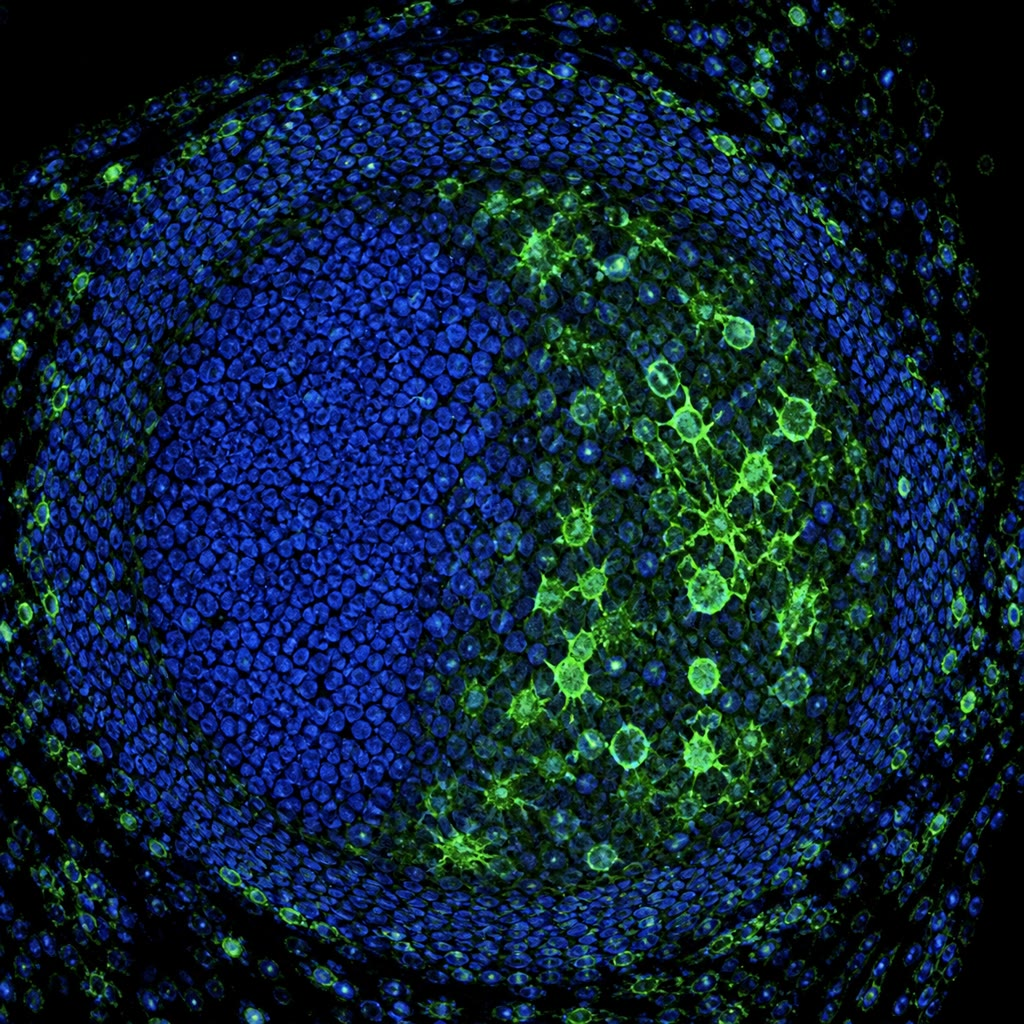
\includegraphics[width=0.36\linewidth]{images/book5/ai/b5-16-germinal-centre.jpg}\hspace{0.04\linewidth}
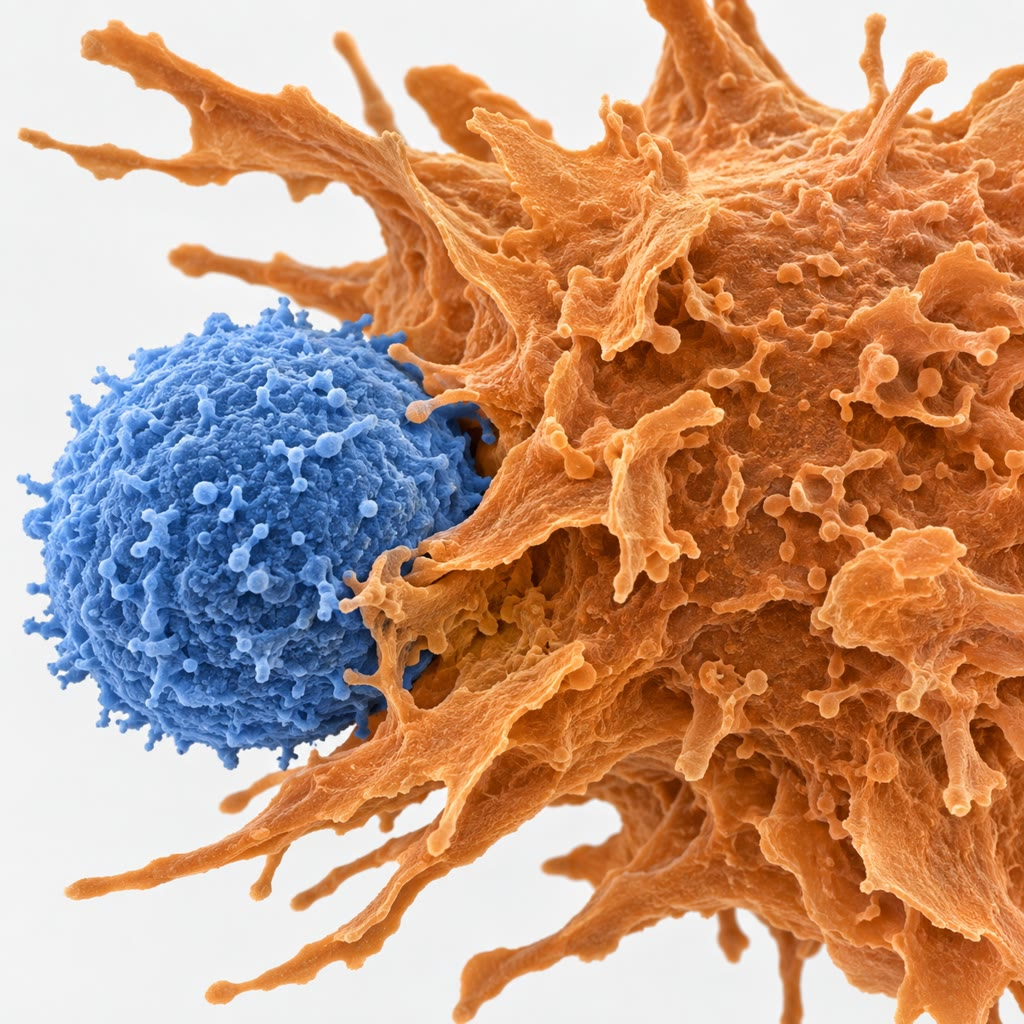
\includegraphics[width=0.36\linewidth]{images/book5/ai/b5-16-t-cell-apc.jpg}

{\small À gauche~: un \omterm{def:b3:adaptive-immunity:germinal-centre}{centre germinatif} dans un \omterm{def:b3:adaptive-immunity:lymphocytes}{ganglion lymphatique} ---
la zone sombre encombrée et la zone plus claire de la sélection. À
droite~: un \omterm{def:b3:adaptive-immunity:lymphocytes}{lymphocyte}~T (petit) au contact d'une \omterm{def:b3:innate-immunity:innate}{cellule dendritique},
le moment où se décide la réponse adaptative.}
\end{omfigure}

\section{La tolérance et ses échecs}

\begin{definition}[La tolérance]\label{def:b3:adaptive-immunity:tolerance}
\index{tolérance}\index{sélection négative}\index{thymus}\index{anergie}\index{FoxP3}\index{auto-immunité}
Le répertoire est fait au hasard et contient donc des récepteurs du soi.
La \emph{tolérance centrale} les retire là où les cellules mûrissent~:
dans le thymus, les \omterm{def:b3:adaptive-immunity:lymphocytes}{lymphocytes}~T dont les récepteurs lient trop
fortement le peptide--CMH du soi sont tués (\emph{sélection négative}),
ceux qui ne peuvent lier le CMH du tout sont tués aussi (ils seraient
inutiles), et seuls les quelques pour cent intermédiaires en sortent~;
un facteur de transcription, AIRE, fait exprimer aux cellules thymiques
des protéines de tous les tissus --- insuline, thyroglobuline --- pour
que les \omterm{def:b3:adaptive-immunity:lymphocytes}{lymphocytes}~T qui leur sont spécifiques puissent y être
éliminés. Les \omterm{def:b3:adaptive-immunity:lymphocytes}{lymphocytes}~B qui lient le soi dans la moelle sont
éliminés ou corrigent leurs récepteurs. La \emph{tolérance périphérique}
gère le reste~: un \omterm{def:b3:adaptive-immunity:lymphocytes}{lymphocyte}~T qui rencontre son \omterm{def:b3:adaptive-immunity:lymphocytes}{antigène} sans
\omterm{def:b3:adaptive-immunity:response}{costimulation} est rendu incapable de répondre (\emph{anergie}) ou
éliminé~; et les \omterm{def:b3:adaptive-immunity:lymphocytes}{lymphocytes}~T \emph{régulateurs}, définis par le
facteur FoxP3, suppriment activement les réponses contre le soi et
contre les \omterm{def:b3:adaptive-immunity:lymphocytes}{antigènes} inoffensifs comme les aliments et les commensaux.
L'\emph{auto-immunité} est l'échec de ces contrôles~: le diabète de
type~1 (les \omterm{def:b3:adaptive-immunity:lymphocytes}{lymphocytes}~T détruisent les cellules $\beta$), la sclérose
en plaques (la myéline), la polyarthrite rhumatoïde (les articulations),
le lupus (des \omterm{def:b3:adaptive-immunity:antibody}{anticorps} contre des composants nucléaires), les maladies
thyroïdiennes~; chacune est associée à des allèles \omterm{def:b3:adaptive-immunity:mhc}{HLA} particuliers, qui
présentent les peptides du soi en cause, et certaines sont déclenchées
par l'infection par un microbe dont les peptides ressemblent à une
protéine du soi (le rhumatisme articulaire aigu après une infection à
streptocoque).
\end{definition}

\begin{proof}[Faits expérimentaux]
Medawar (1953) injecta des cellules d'une souche consanguine de souris à
des souriceaux nouveau-nés d'une autre~; devenus adultes, les receveurs
acceptèrent des greffes de peau de la souche donneuse qu'ils auraient
sinon rejetées, tout en rejetant les greffes de souches tierces. La
\omterm{def:b3:adaptive-immunity:tolerance}{tolérance} était acquise, spécifique, et fixée par ce que le système
immunitaire avait rencontré tôt --- la base expérimentale de
l'élimination burnétienne des clones autoréactifs. Les enfants nés sans
gène AIRE fonctionnel développent une \omterm{def:b3:adaptive-immunity:tolerance}{auto-immunité} contre de nombreux
organes à la fois~; ceux qui sont dépourvus de \omterm{def:b3:adaptive-immunity:tolerance}{FoxP3} (un rare syndrome
lié à l'X) développent une \omterm{def:b3:adaptive-immunity:tolerance}{auto-immunité} mortelle dès la petite enfance
--- les deux bras de la \omterm{def:b3:adaptive-immunity:tolerance}{tolérance}, chacun montré par son absence.
\end{proof}

\begin{example}[Hypersensibilité, déficit, transplantation]\label{ex:b3:adaptive-immunity:failures}
L'\emph{allergie} est une réponse Th2 à un \omterm{def:b3:adaptive-immunity:lymphocytes}{antigène} inoffensif ---
pollen, arachide, pénicilline --- qui produit de l'IgE~; à la
réexposition l'\omterm{def:b3:adaptive-immunity:lymphocytes}{antigène} ponte les IgE des mastocytes, qui libèrent
l'histamine en quelques minutes, et si l'\omterm{def:b3:adaptive-immunity:lymphocytes}{antigène} est dans le sang la
libération systémique est l'\emph{anaphylaxie}, traitée par
l'adrénaline. \emph{Déficit immunitaire}~: les enfants dépourvus de \omterm{def:b3:adaptive-immunity:antibody}{RAG}
ou de l'enzyme ADA ne font aucun \omterm{def:b3:adaptive-immunity:lymphocytes}{lymphocyte} (déficit immunitaire combiné
sévère) et meurent d'infection à moins de recevoir une greffe de moelle
ou une thérapie génique~; le VIH détruit les \omterm{def:b3:adaptive-immunity:lymphocytes}{lymphocytes}~T CD4 et avec
eux l'aide dont toute réponse a besoin. \emph{Transplantation}~: les
\omterm{def:b3:adaptive-immunity:lymphocytes}{lymphocytes}~T du receveur voient les molécules \omterm{def:b3:adaptive-immunity:mhc}{HLA} du donneur comme
étrangères, et jusqu'à un dixième de tous les \omterm{def:b3:adaptive-immunity:lymphocytes}{lymphocytes}~T répondent
--- bien plus que pour aucun pathogène --- de sorte qu'on apparie les
greffons aux loci \omterm{def:b3:adaptive-immunity:mhc}{HLA} et qu'on immunodéprime le receveur à vie~; une
greffe de moelle peut au contraire attaquer son nouvel hôte. Et les
usages délibérés~: les \omterm{def:b3:adaptive-immunity:antibody}{anticorps} monoclonaux du
\cref{ch:b3:genetic-engineering}, les \omterm{prop:b3:cancer-biology:immune}{inhibiteurs de point de contrôle}
qui lâchent les \omterm{def:b3:adaptive-immunity:lymphocytes}{lymphocytes}~T contre les \omterm{def:b3:cancer-biology:hallmarks}{tumeurs}
(\cref{ch:b3:cancer-biology}), et les \omterm{def:b3:adaptive-immunity:lymphocytes}{lymphocytes}~T équipés d'un
récepteur chimérique d'\omterm{def:b3:adaptive-immunity:lymphocytes}{antigène} tumoral (CAR-T), qui ont guéri des
leucémies que rien d'autre ne touchait.
\end{example}

\section{La vaccination}

\begin{definition}[Les vaccins et l'immunité de groupe]\label{def:b3:adaptive-immunity:vaccine}
\index{vaccin}\index{immunité de groupe}\index{nombre de reproduction de base}\index{efficacité vaccinale}
Un \emph{vaccin} présente des \omterm{def:b3:adaptive-immunity:lymphocytes}{antigènes} d'un pathogène, avec un adjuvant
ou sous une forme qui déclenche les récepteurs innés, de sorte que celui
qui le reçoit acquiert des \omterm{def:b3:adaptive-immunity:response}{cellules mémoires} et des \omterm{def:b3:adaptive-immunity:antibody}{anticorps} sans la
maladie (le \cref{ch:b3:virology} en énumère les sortes). Son
\emph{efficacité} $E$ est la fraction des personnes vaccinées qui sont
protégées. La protection s'étend au-delà des vaccinés~: un pathogène qui
se propage dans une population où chaque cas en infecte $R_{0}$ autres
en moyenne quand tous sont susceptibles --- le \emph{nombre de
reproduction de base} --- n'en infecte que $R_{0}$ fois la fraction
susceptible quand certains sont immuns, et s'éteint quand ce nombre
tombe sous un. C'est l'\emph{immunité de groupe}~: au-delà d'un seuil de
personnes immunes la chaîne de transmission se rompt et les non-vaccinés
--- nourrissons, immunodéprimés, ceux chez qui le vaccin a échoué ---
sont protégés par les autres.
\end{definition}

\begin{theorem}[Le seuil d'immunité de groupe]\label{thm:b3:adaptive-immunity:herd}
\index{immunité de groupe!seuil}\index{modèle SIR}
Dans une population où une fraction $p$ est immune et le reste
susceptible, chaque cas infecte en moyenne $R_{\text{eff}} = R_{0}(1 -
p)$ autres personnes. Une épidémie ne peut démarrer si
$R_{\text{eff}} < 1$, c'est-à-dire si
\[
p > p_{c} = 1 - \frac{1}{R_{0}} .
\]
Avec un \omterm{def:b3:adaptive-immunity:vaccine}{vaccin} d'efficacité $E$, la couverture nécessaire est $f_{c} = p_{c}/E$.
Si une épidémie se déroule bel et bien dans une population susceptible
(le \omterm{thm:b3:adaptive-immunity:herd}{modèle SIR}, avec un taux d'infection $\beta$ et un taux de guérison
$\gamma$, $R_{0} =
\beta/\gamma$), elle culmine quand la fraction susceptible est tombée à
$1/R_{0}$, et la fraction jamais infectée, $s_{\infty}$, vérifie
$\ln s_{\infty} = -R_{0}(1 - s_{\infty})$.
\end{theorem}
\begin{proof}
Chaque cas noue des contacts qui infecteraient $R_{0}$ personnes si
toutes étaient susceptibles~; une fraction $1 - p$ d'entre elles l'est,
donc $R_{\text{eff}} =
R_{0}(1-p)$, et la condition $R_{\text{eff}} < 1$ donne $p_{c}$~; un
\omterm{def:b3:adaptive-immunity:vaccine}{vaccin} qui protège une fraction $E$ de ceux qui le reçoivent rend immune
une fraction $Ef$ de la population, donc $Ef > p_{c}$. Dans le \omterm{thm:b3:adaptive-immunity:herd}{modèle
SIR}, $\mathrm{d}s/\mathrm{d}t = -\beta si$ et $\mathrm{d}i/\mathrm{d}t =
\beta si - \gamma i = \gamma i(R_{0}s - 1)$, donc $i$ croît tant que $s >
1/R_{0}$ et décroît ensuite~: le pic est en $s = 1/R_{0}$. En divisant
les deux équations, $\mathrm{d}i/\mathrm{d}s = -1 + 1/(R_{0}s)$, donc $i + s -
\ln s/R_{0}$ est constant~; en l'évaluant au début ($s = 1$, $i
\approx 0$) et à la fin ($i = 0$, $s = s_{\infty}$) on obtient
$s_{\infty} - \ln s_{\infty}/R_{0} = 1$, la relation de taille finale.
\end{proof}

\begin{example}[La rougeole et la variole]\label{ex:b3:adaptive-immunity:measles}
La rougeole a $R_{0} \approx 15$~: $p_{c} = 1 - 1/15 = 93\,\%$, et avec
un \omterm{def:b3:adaptive-immunity:vaccine}{vaccin} d'efficacité $97\,\%$ après deux doses la couverture
nécessaire est de $96\,\%$ --- ce qui explique pourquoi la rougeole
revient partout où la vaccination glisse de quelques pour cent, et
pourquoi un enfant non vacciné d'un pays bien vacciné est malgré tout en
sécurité. La variole avait $R_{0} \approx 5$--$7$, un seuil proche de
$80$--$85\,\%$, aucun réservoir animal, aucun porteur asymptomatique et
un \omterm{def:b3:adaptive-immunity:vaccine}{vaccin} qui marchait en une dose~: éradicable, et éradiquée. La
poliomyélite y est presque. La grippe et les coronavirus, dont les
\omterm{def:b3:adaptive-immunity:lymphocytes}{antigènes} dérivent (\cref{ch:b3:virology}) et dont l'immunité s'estompe,
ne le sont pas. Dans une population non vaccinée une épidémie avec
$R_{0} = 3$ infecte, par la relation de taille finale,
$1 - s_{\infty} = 94\,\%$ des gens~; avec $R_{0} = 1.5$, $58\,\%$.
\end{example}

\begin{omfigure}
\begin{tikzpicture}
\begin{axis}[
  width=6.4cm, height=5.4cm,
  axis x line=bottom, axis y line=left,
  xmin=1, xmax=18, ymin=0, ymax=1,
  xlabel={$R_{0}$}, ylabel={seuil $p_{c}$},
  xlabel style={font=\small, at={(axis description cs:0.5,-0.12)}, anchor=north}, ylabel style={font=\small},
  tick label style={font=\scriptsize}, xtick={1,3,6,9,12,15,18}, ytick={0,0.5,0.8,0.93,1}, yticklabels={0,0.5,0.8,0.93,1},
  clip=false,
]
\addplot[very thick, omDef, domain=1:18, samples=80] {1-1/x};
\fill[omThm] (axis cs:15,0.933) circle (2pt); \node[font=\scriptsize, anchor=south east] at (axis cs:15,0.94) {rougeole};
\fill[omThm] (axis cs:6,0.833) circle (2pt); \node[font=\scriptsize, anchor=north west] at (axis cs:6.3,0.82) {variole};
\fill[omThm] (axis cs:2.5,0.6) circle (2pt); \node[font=\scriptsize, anchor=north west] at (axis cs:2.6,0.58) {grippe de 1918};
\end{axis}
\begin{axis}[
  at={(7.6cm,0)}, anchor=south west,
  width=6.4cm, height=5.4cm,
  axis x line=bottom, axis y line=left,
  xmin=0, xmax=60, ymin=0, ymax=0.35,
  xlabel={jours}, ylabel={fraction infectieuse},
  xlabel style={font=\small, at={(axis description cs:0.5,-0.12)}, anchor=north}, ylabel style={font=\small},
  tick label style={font=\scriptsize}, xtick={0,20,40,60}, ytick={0,0.1,0.2,0.3},
  clip=false,
]
\addplot[very thick, omThm, smooth] coordinates {(0,0.001) (5,0.003) (10,0.012) (15,0.04) (20,0.12) (25,0.25) (28,0.30) (31,0.27) (35,0.18) (40,0.09) (45,0.04) (50,0.015) (55,0.006) (60,0.002)};
\addplot[very thick, omDef, smooth] coordinates {(0,0.001) (5,0.0015) (10,0.0025) (15,0.004) (20,0.006) (25,0.009) (30,0.012) (35,0.014) (40,0.015) (45,0.014) (50,0.012) (55,0.009) (60,0.007)};
\node[font=\scriptsize, omThm, anchor=west] at (axis cs:30,0.3) {aucune immunité, $R_{0} = 3$};
\node[font=\scriptsize, omDef, anchor=south west] at (axis cs:32,0.03) {\qty{60}{\%} de vaccinés~: $R_{\text{eff}} = 1.2$};
\end{axis}
\end{tikzpicture}

{\small À gauche~: le seuil $1 - 1/R_{0}$ --- plus la maladie est
contagieuse, plus il faut que tout le monde, ou presque, soit immun. À
droite~: une épidémie SIR avec $R_{0} = 3$ dans une population naïve et
dans une population immune à \qty{60}{\%}, ce qui ne suffit pas à
l'arrêter mais l'aplatit et la ralentit.}
\end{omfigure}

\begin{omfigure}
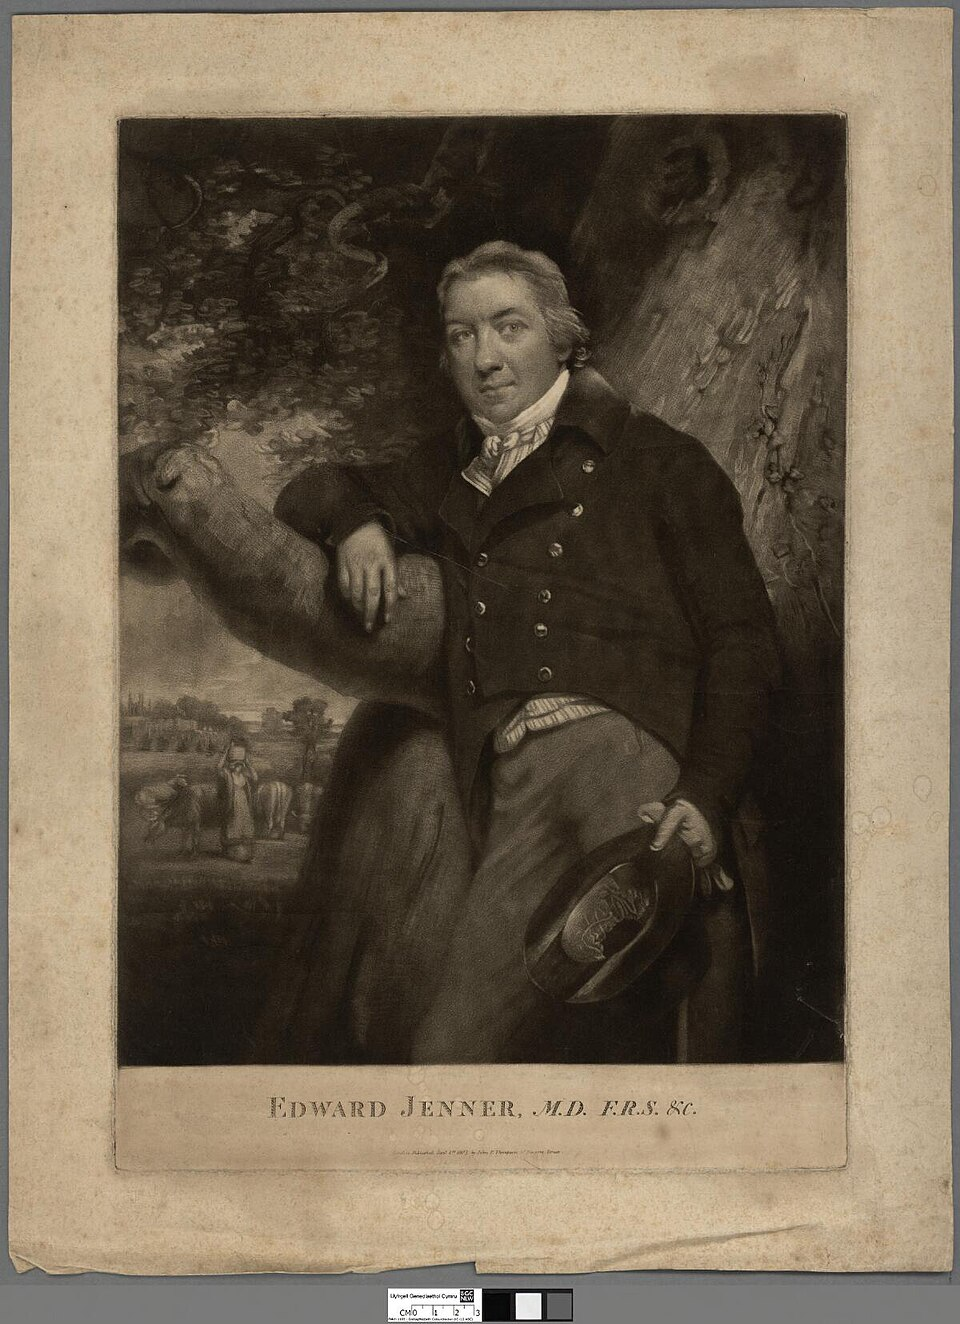
\includegraphics[width=0.30\linewidth]{images/book5/jenner.jpg}\hspace{0.04\linewidth}
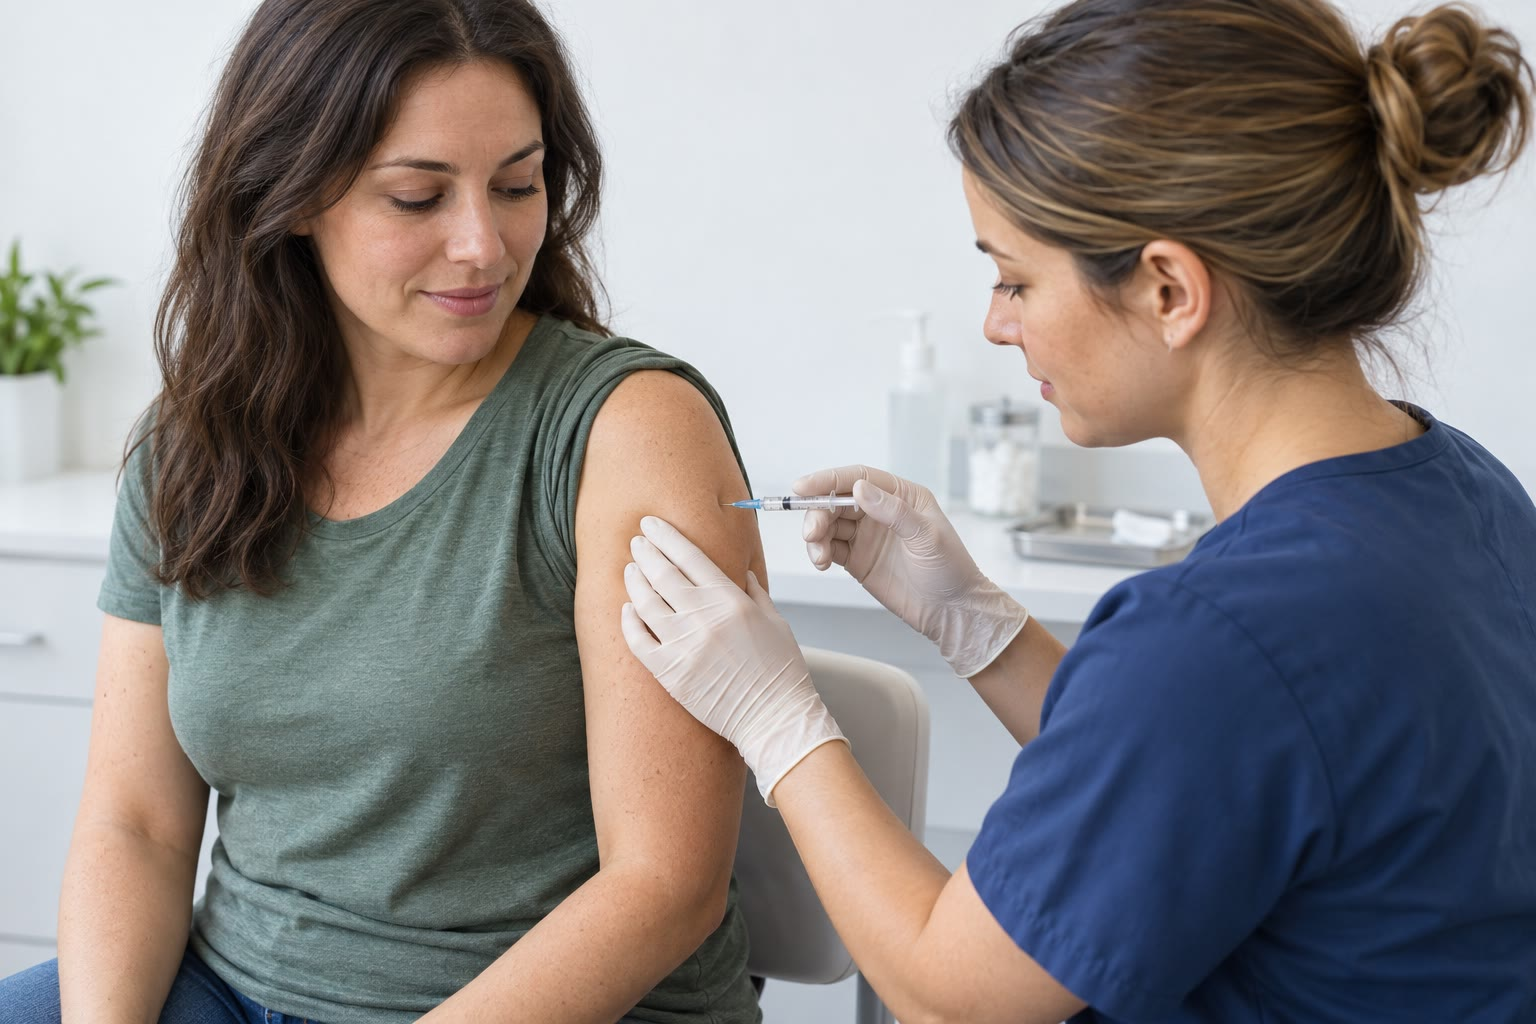
\includegraphics[width=0.50\linewidth]{images/book5/ai/b5-16-vaccination.jpg}

{\small Edward Jenner, qui protégea en 1796 un garçon contre la variole
au moyen de la vaccine et fonda la vaccination (gravure de 1807, domaine
public). À droite~: le même geste deux siècles plus tard --- un \omterm{def:b3:adaptive-immunity:vaccine}{vaccin}
intramusculaire, dont les \omterm{def:b3:innate-immunity:innate}{cellules dendritiques} du deltoïde porteront
l'\omterm{def:b3:adaptive-immunity:lymphocytes}{antigène} aux ganglions axillaires.}
\end{omfigure}

\begin{remark}[Ce dont l'immunité se souvient]\label{rem:b3:adaptive-immunity:memory}
Le système immunitaire adaptatif est une machine darwinienne logée en
chacun de nous~: variation au hasard (V(D)J, hypermutation), sélection
(par l'\omterm{def:b3:adaptive-immunity:lymphocytes}{antigène}, dans le \omterm{def:b3:adaptive-immunity:germinal-centre}{centre germinatif}, contre le soi dans le
\omterm{def:b3:adaptive-immunity:tolerance}{thymus}) et hérédité (\omterm{def:b3:adaptive-immunity:response}{cellules mémoires}, expansion clonale). Il résout en
quelques semaines le problème que l'évolution résout en millénaires ---
une molécule qui lie une cible jamais vue --- et ses réponses comptent
parmi les cas d'évolution les mieux étudiés qu'on ait observés
directement. Son coût est l'\omterm{def:b3:adaptive-immunity:tolerance}{auto-immunité}, sa dépendance au jugement du
système inné est absolue, et sa mémoire, que Jenner a exploitée et que
les \omterm{def:b3:adaptive-immunity:vaccine}{vaccins} écrivent délibérément, est la raison pour laquelle une
espèce d'animaux à longue vie et à reproduction lente peut survivre dans
un monde de microbes à reproduction rapide.
\end{remark}

\section{Exercices}

\begin{exercise}[$\star$]\label{exo:b3:adaptive-immunity:1}
Énoncer les quatre principes de la \omterm{def:b3:adaptive-immunity:lymphocytes}{sélection clonale} et l'expérience qui
appuie chacun des deux premiers.
\end{exercise}

\begin{exercise}[$\star$]\label{exo:b3:adaptive-immunity:2}
Décrire la structure d'un \omterm{def:b3:adaptive-immunity:antibody}{anticorps} et donner la fonction de chacune des
cinq classes.
\end{exercise}

\begin{exercise}[$\star$]\label{exo:b3:adaptive-immunity:3}
Opposer le \omterm{def:b3:adaptive-immunity:mhc}{CMH de classe~I} et celui de classe~II par la distribution
cellulaire, la source du peptide, la longueur du peptide et le
\omterm{def:b3:adaptive-immunity:lymphocytes}{lymphocyte}~T qui lit chacun.
\end{exercise}

\begin{exercise}[$\star$]\label{exo:b3:adaptive-immunity:4}
Définir $R_{0}$ et le seuil d'\omterm{def:b3:adaptive-immunity:vaccine}{immunité de groupe}, et calculer le seuil
pour les oreillons ($R_{0} = 5$), la coqueluche ($R_{0} = 12$) et la
grippe de 1918 ($R_{0} = 2.5$).
\end{exercise}

\begin{exercise}[$\star\star$]\label{exo:b3:adaptive-immunity:5}
Une espèce a $V_{H} = 50$, $D = 20$, $J_{H} = 5$ et un seul locus léger
avec $V = 60$, $J = 4$. Calculer le répertoire combinatoire, puis le
total avec un facteur jonctionnel de $10^{4}$. Comment se compare-t-il
aux $10^{9}$ \omterm{def:b3:adaptive-immunity:lymphocytes}{lymphocytes}~B de l'animal~?
\end{exercise}

\begin{exercise}[$\star\star$]\label{exo:b3:adaptive-immunity:6}
La région variable d'un \omterm{def:b3:adaptive-immunity:lymphocytes}{lymphocyte}~B de \omterm{def:b3:adaptive-immunity:germinal-centre}{centre germinatif} fait
\qty{1000}{bp}~; AID mute à $10^{-3}$ par paire de bases et par
division. Sur $20$ divisions, combien de mutations par cellule, et parmi
$10^{5}$ cellules combien de variants distincts de l'\omterm{def:b3:adaptive-immunity:antibody}{anticorps} à une
base sont engendrés~? Comparer aux $3000$ substitutions simples
possibles.
\end{exercise}

\begin{exercise}[$\star\star$]\label{exo:b3:adaptive-immunity:7}
Expliquer pourquoi un \omterm{def:b3:adaptive-immunity:lymphocytes}{lymphocyte}~T d'une personne ne reconnaît pas les
peptides viraux présentés par les cellules d'une autre, et pourquoi ce
même fait rend les greffes difficiles et le système \omterm{def:b3:adaptive-immunity:mhc}{HLA} polymorphe.
\end{exercise}

\begin{exercise}[$\star\star$]\label{exo:b3:adaptive-immunity:8}
Prévoir le phénotype immunitaire d'un enfant dépourvu (a) de RAG1, (b)
d'AIRE, (c) de \omterm{def:b3:adaptive-immunity:tolerance}{FoxP3}, (d) de l'enzyme de commutation AID, et (e) de
\omterm{def:b3:adaptive-immunity:lymphocytes}{lymphocytes}~T CD4.
\end{exercise}

\begin{exercise}[$\star\star$]\label{exo:b3:adaptive-immunity:9}
Un \omterm{def:b3:adaptive-immunity:vaccine}{vaccin} a une efficacité de \qty{90}{\%} et la maladie $R_{0} = 6$.
Quelle couverture arrête la transmission~? Si la couverture est de
\qty{80}{\%}, que vaut $R_{\text{eff}}$, et quelle fraction de la
population une épidémie infecte-t-elle (utiliser la relation de taille
finale avec $R_{0}$ remplacé par $R_{\text{eff}}$ parmi les
susceptibles --- ou dire pourquoi c'est approximativement juste)~?
\end{exercise}

\begin{exercise}[$\star\star\star$]\label{exo:b3:adaptive-immunity:10}
Établir la relation de taille finale du théorème à partir des équations
SIR et la résoudre numériquement pour $R_{0} = 1.5$, $2$, $3$ et $5$.
Pourquoi une épidémie n'infecte-t-elle jamais tout le monde, même sans
aucune intervention~?
\end{exercise}

\begin{exercise}[$\star\star\star$]\label{exo:b3:adaptive-immunity:11}
La \omterm{def:b3:adaptive-immunity:germinal-centre}{maturation d'affinité} multiplie la liaison par mille en trois
semaines. Traiter le \omterm{def:b3:adaptive-immunity:germinal-centre}{centre germinatif} comme une population sous
sélection~: avec un taux de mutation d'une par cellule et par division,
une fraction $10^{-2}$ des mutations améliorant l'affinité d'un facteur
$1.5$ et le reste neutre ou nuisible, combien de tours de sélection
faut-il pour un gain d'un facteur mille, et combien de cellules chaque
tour doit-il cribler~? Commenter le fait que le \omterm{def:b3:adaptive-immunity:germinal-centre}{centre germinatif} soit
organisé en cycles.
\end{exercise}

\begin{exercise}[$\star\star\star$]\label{exo:b3:adaptive-immunity:12}
Les maladies auto-immunes sont plus fréquentes chez la femme et
associées à des allèles \omterm{def:b3:adaptive-immunity:mhc}{HLA}~; le diabète de type~1 a été multiplié par
cinq en cinquante ans dans les pays riches. Proposer, avec les
mécanismes de ce chapitre et du \cref{ch:b3:microbiomes}, une
explication de chaque observation et un test de chacune.
\end{exercise}

\section{Problème~: une campagne de vaccination}

\begin{problem}[{Problème du week-end --- un répertoire dénombré, une
réponse chronométrée de cent cellules à un millilitre de sérum, un
centre germinatif mené comme un algorithme évolutif, et une campagne
contre la rougeole planifiée face au seuil de groupe, pour finir sur la
taille du répertoire, l'anticorps qu'un plasmocyte fabrique en un jour
et la couverture dont un pays a besoin}]
\label{pb:b3:adaptive-immunity:1}
Données~: $V_{H} = 40$, $D = 25$, $J_{H} = 6$~; loci légers $(40, 5)$ et
$(30, 4)$~; facteur jonctionnel $3\times 10^{4}$. Un corps a $10^{11}$
\omterm{def:b3:adaptive-immunity:lymphocytes}{lymphocytes}~B~; un sur $10^{5}$ lie un épitope donné~; $100$ précurseurs
sont recrutés~; division toutes les \qty{8}{h} pendant $7$ jours~;
\qty{30}{\%} du clone devient des \omterm{def:b3:adaptive-immunity:response}{plasmocytes} sécrétant chacun $2000$
molécules d'IgG par seconde~; l'IgG fait \qty{150}{kDa}~; volume
plasmatique \qty{3}{L}~; demi-vie de l'IgG \qty{21}{d}. \omterm{def:b3:adaptive-immunity:germinal-centre}{Centre
germinatif}~: région variable de \qty{1000}{bp}, $10^{-3}$ mutation par
pb et par division, une mutation sur $100$ améliore l'affinité d'un
facteur $1.5$. Rougeole~: $R_{0} = 15$, \omterm{def:b3:adaptive-immunity:vaccine}{efficacité vaccinale} $0.93$
après une dose et $0.97$ après deux~; un pays de $5\times 10^{6}$
habitants avec $60\,000$ naissances par an.

\medskip
\noindent\textbf{Partie I --- Le répertoire.}
\begin{enumerate}
  \item Calculer le répertoire combinatoire et le total avec la
        \omterm{def:b3:adaptive-immunity:antibody}{diversité jonctionnelle}.
  \item Comparer au nombre de \omterm{def:b3:adaptive-immunity:lymphocytes}{lymphocytes}~B. Quelle fraction du
        répertoire possible un corps exprime-t-il à un instant donné, et
        qu'en découle-t-il pour les répertoires de deux individus~?
  \item Combien de \omterm{def:b3:adaptive-immunity:lymphocytes}{lymphocytes}~B du corps lient l'épitope~? Combien, en
        moyenne, dans un ganglion contenant $10^{8}$ \omterm{def:b3:adaptive-immunity:lymphocytes}{lymphocytes}~B~?
  \item Un nouveau-né a $10^{9}$ \omterm{def:b3:adaptive-immunity:lymphocytes}{lymphocytes}~B. Combien lient l'épitope,
        et pourquoi la réponse d'un nouveau-né est-elle faible malgré
        tout~?
  \item La troisième boucle de la chaîne lourde d'un \omterm{def:b3:adaptive-immunity:antibody}{anticorps} est faite
        par la \omterm{def:b3:adaptive-immunity:antibody}{diversité jonctionnelle}. Expliquer pourquoi cette boucle
        est la partie la plus variable de la molécule et se trouve
        d'ordinaire au centre du site de liaison.
  \item L'\omterm{def:b3:adaptive-immunity:germinal-centre}{hypermutation somatique} ajoute de la diversité après la
        sélection, la V(D)J avant. Pourquoi est-il avantageux d'avoir
        les deux, dans cet ordre~?
\end{enumerate}

\medskip
\noindent\textbf{Partie II --- La réponse.}
\begin{enumerate}[resume]
  \item À partir de $100$ cellules se divisant toutes les \qty{8}{h},
        combien après $7$ jours~? Combien de \omterm{def:b3:adaptive-immunity:response}{plasmocytes}~?
  \item Combien de molécules d'IgG sécrètent-ils par jour, et quelle
        masse~? Quelle concentration sérique la production d'un jour
        donne-t-elle dans \qty{3}{L}~?
  \item Après dix jours de sécrétion à ce rythme, en négligeant la
        décroissance, quelle est la concentration en g/L~? Comparer à
        l'IgG totale normale de \qty{10}{g/L}.
  \item Les \omterm{def:b3:adaptive-immunity:response}{plasmocytes} meurent au bout de deux semaines~; l'\omterm{def:b3:adaptive-immunity:antibody}{anticorps}
        décroît alors avec une demi-vie de \qty{21}{d}. Combien de temps
        avant que la concentration de la question 9 tombe d'un facteur
        cent~? Qu'est-ce qui entretient l'\omterm{def:b3:adaptive-immunity:antibody}{anticorps} pendant des années~?
  \item Une réponse secondaire part de $10^{5}$ \omterm{def:b3:adaptive-immunity:response}{cellules mémoires}.
        Combien de cellules après $3$ jours, et comment cela se
        compare-t-il à la réponse primaire au jour 3 et au jour 7~?
  \item Expliquer pourquoi l'IgM vient d'abord et l'IgG ensuite dans une
        réponse primaire, et pourquoi la réponse secondaire est d'emblée
        une IgG.
\end{enumerate}

\medskip
\noindent\textbf{Partie III --- Le \omterm{def:b3:adaptive-immunity:germinal-centre}{centre germinatif}.}
\begin{enumerate}[resume]
  \item Combien de mutations un \omterm{def:b3:adaptive-immunity:lymphocytes}{lymphocyte}~B acquiert-il dans sa région
        variable par division~? Sur $20$ divisions~?
  \item Quelle fraction des filles d'une division porte une mutation
        améliorante~? Dans un \omterm{def:b3:adaptive-immunity:germinal-centre}{centre germinatif} de $10^{4}$ cellules en
        division, combien de cellules améliorées apparaissent par
        division~?
  \item Combien d'améliorations successives d'un facteur $1.5$ donnent
        un gain d'affinité d'un facteur mille~? Si chaque tour de
        sélection prend deux divisions (\qty{12}{h}), combien de temps
        cela fait-il~?
  \item La plupart des mutations abîment l'\omterm{def:b3:adaptive-immunity:antibody}{anticorps}. Si \qty{50}{\%}
        des mutations détruisent la liaison, quelle fraction des
        cellules survit à la mutation de chaque division, et pourquoi la
        zone claire doit-elle tuer la plupart des cellules~?
  \item Un \omterm{def:b3:adaptive-immunity:vaccine}{vaccin} donné en deux doses espacées de six semaines produit
        des \omterm{def:b3:adaptive-immunity:antibody}{anticorps} de meilleure affinité qu'une dose. Expliquer par
        le \omterm{def:b3:adaptive-immunity:germinal-centre}{centre germinatif}.
  \item Certains \omterm{def:b3:virology:virus}{virus} (VIH, grippe) échappent aux \omterm{def:b3:adaptive-immunity:antibody}{anticorps} en mutant
        leur surface. Expliquer pourquoi le \omterm{def:b3:adaptive-immunity:germinal-centre}{centre germinatif} est
        néanmoins le fondement de l'espoir d'un \omterm{def:b3:adaptive-immunity:vaccine}{vaccin} largement
        protecteur.
\end{enumerate}

\medskip
\noindent\textbf{Partie IV --- La campagne.}
\begin{enumerate}[resume]
  \item Seuil de groupe pour la rougeole, et couverture requise avec une
        dose~; avec deux doses.
  \item Le pays vaccine \qty{90}{\%} des enfants avec deux doses.
        Fraction immune, $R_{\text{eff}}$, et le verdict~: la rougeole
        circule-t-elle~?
  \item Combien d'enfants susceptibles s'accumulent par année de
        naissances à \qty{90}{\%} de couverture (non vaccinés plus
        échecs vaccinaux)~? Après cinq ans sans rougeole, combien y
        a-t-il de susceptibles, et pourquoi une importation cause-t-elle
        alors une flambée~?
  \item Utiliser la relation de taille finale avec le nombre de
        reproduction effectif parmi les susceptibles pour estimer la
        fraction de ces susceptibles qu'une flambée infecte. (Prendre
        $R_{\text{eff}}$ de la question 20 comme nombre de reproduction
        dans la population entière, et noter que dans le réservoir
        susceptible la maladie se propage comme si $R_{0}$ valait
        $R_{\text{eff}}$.)
  \item La couverture est portée à \qty{95}{\%} avec deux doses.
        Fraction immune et $R_{\text{eff}}$~; le seuil est-il atteint~?
  \item Les nourrissons de moins d'un an ne peuvent être vaccinés contre
        la rougeole et sont les plus susceptibles d'en mourir. Expliquer
        comment la campagne les protège, et ce qu'il advient de leur
        protection si la couverture tombe à \qty{85}{\%}.
  \item Résumer~: le répertoire total (question~1), l'IgG que les
        \omterm{def:b3:adaptive-immunity:response}{plasmocytes} d'un jour fabriquent (question~8), et la couverture
        à deux doses dont le pays a besoin (question~19).
\end{enumerate}
\end{problem}
